\begingroup
\RaggedRight

Hardware Trojan (HT) insertion involves a malicious alteration to a hardware component's design, posing risks such as device malfunction, data leakage, or physical damage \cite{francq2015introduction}. With the semiconductor industry adopting a fabless model, the potential for HT insertion at various manufacturing stages grows, posing a substantial security threat. Traditional detection methods, like signature-based approaches \cite{gbade2014signature}, prove ineffective against evolving HT attacks, prompting a shift towards Machine Learning (ML) solutions. However, existing ML approaches often lack information on datasets, struggle with concept drift, and require additional evaluation metrics \cite{285613}. A study in \cite{quiring2022and} questions the universality of ML in addressing hardware security concerns \cite{liu2021two}.

ML methods face challenges due to concept drift caused by intelligent modifications to HT insertion techniques. The paper introduces \textbf{PALETTE}, an algorithm-agnostic framework for evolving hardware Trojan detection, utilizing conformal prediction \cite{shafer2008tutorial}. It provides risk-aware theoretical guaranteed coverage under covariate shift \cite{tibshirani2019conformal}. Non-invasive and applicable as a wrapper over existing ML models, \textbf{PALETTE} offers set predictions, ensuring the correct class is included 95\% of the time on average (i.e., $\alpha$ = 0.05).

HT insertion is a concern in fabless semiconductor manufacturing, with potential attacks at different stages \cite{salmani2017hardware, Regazzoni:HTDetection, Guin:HTDetection, Salmani:HTDetection}. Vulnerabilities span design phases, EDA processes, and post-production stages, necessitating robust security measures \cite{narasimhan2011tesr, muralidhar2021contrastive, chang2023supplier, panduro2023effective, monjur2023hardware}. Comprehensive approaches, while crucial, come with drawbacks, leading to the relevance of ML in countering HTs. Challenges like resource-intensive training, adversarial attacks, and interpretability are acknowledged.

ML has emerged as a potent tool for HT detection in fabless semiconductor manufacturing \cite{gubbi2023hardware, huang2020survey, liakos2019machine, koblah2023survey, koylu2023survey}. Challenges include acquiring diverse datasets, susceptibility to adversarial attacks \cite{west2023towards}, and the need for interpretability and explainability \cite{li2022interpretable, caruana2020intelligible}. \textbf{NOODLE}, proposed in this paper, is an uncertainty-aware hardware Trojan detection using multimodal deep learning with graph representation and tabular data, performing binary classification.

\section*{Research Gap}

The shared identification of these gaps in research sets the stage for a thorough exploration plan, underscoring the particular areas that demand deeper investigation and focused development in the field of multimodal learning for detecting hardware trojans. A few of them are discussed below:

\begin{itemize}

    \item \textbf{Dataset Transparency and Class Distribution:} The lack of transparency in revealing comprehensive dataset details, especially concerning class distribution differences, highlights a research gap. There is a need for scholarly attention to address transparency issues and gain a nuanced understanding of dataset characteristics in the presence of significant class distribution variations.
    
    \item \textbf{Concept Drift in Model Evaluation:} The insufficiency in considering "concept drift" stemming from adversaries' evolving insertion techniques introduces a research gap. Coping strategies are required to effectively handle concept drift, indicating the necessity for further exploration and validation in this area.
    
    \item \textbf{Additional Measures for Model Evaluation:} The inadequacy of conventional metrics for model evaluation underscores a research gap. There is a need for additional measures to strengthen traditional evaluation methods, ensuring reliable decision-making and comprehensive prediction coverage.
    
    
    \item \textbf{Uncertainty-Aware Multimodal Learning:} The limited exploration of diverse multimodal approaches, particularly beyond prevalent graph representation and tabular data, is identified as a research gap. Scholarly inquiry and investigation into various modality combinations in multimodal learning for hardware trojan detection are needed.
    

    
    \item \textbf{Interpretability and Explainability:} The acknowledgment of the significance of interpretability and explainability in multimodal models highlights a research gap. The development of interpretable multimodal hardware trojan detection models is necessary to enhance trust and understanding in the domain.

\end{itemize}



\begin{figure}
  \centering
   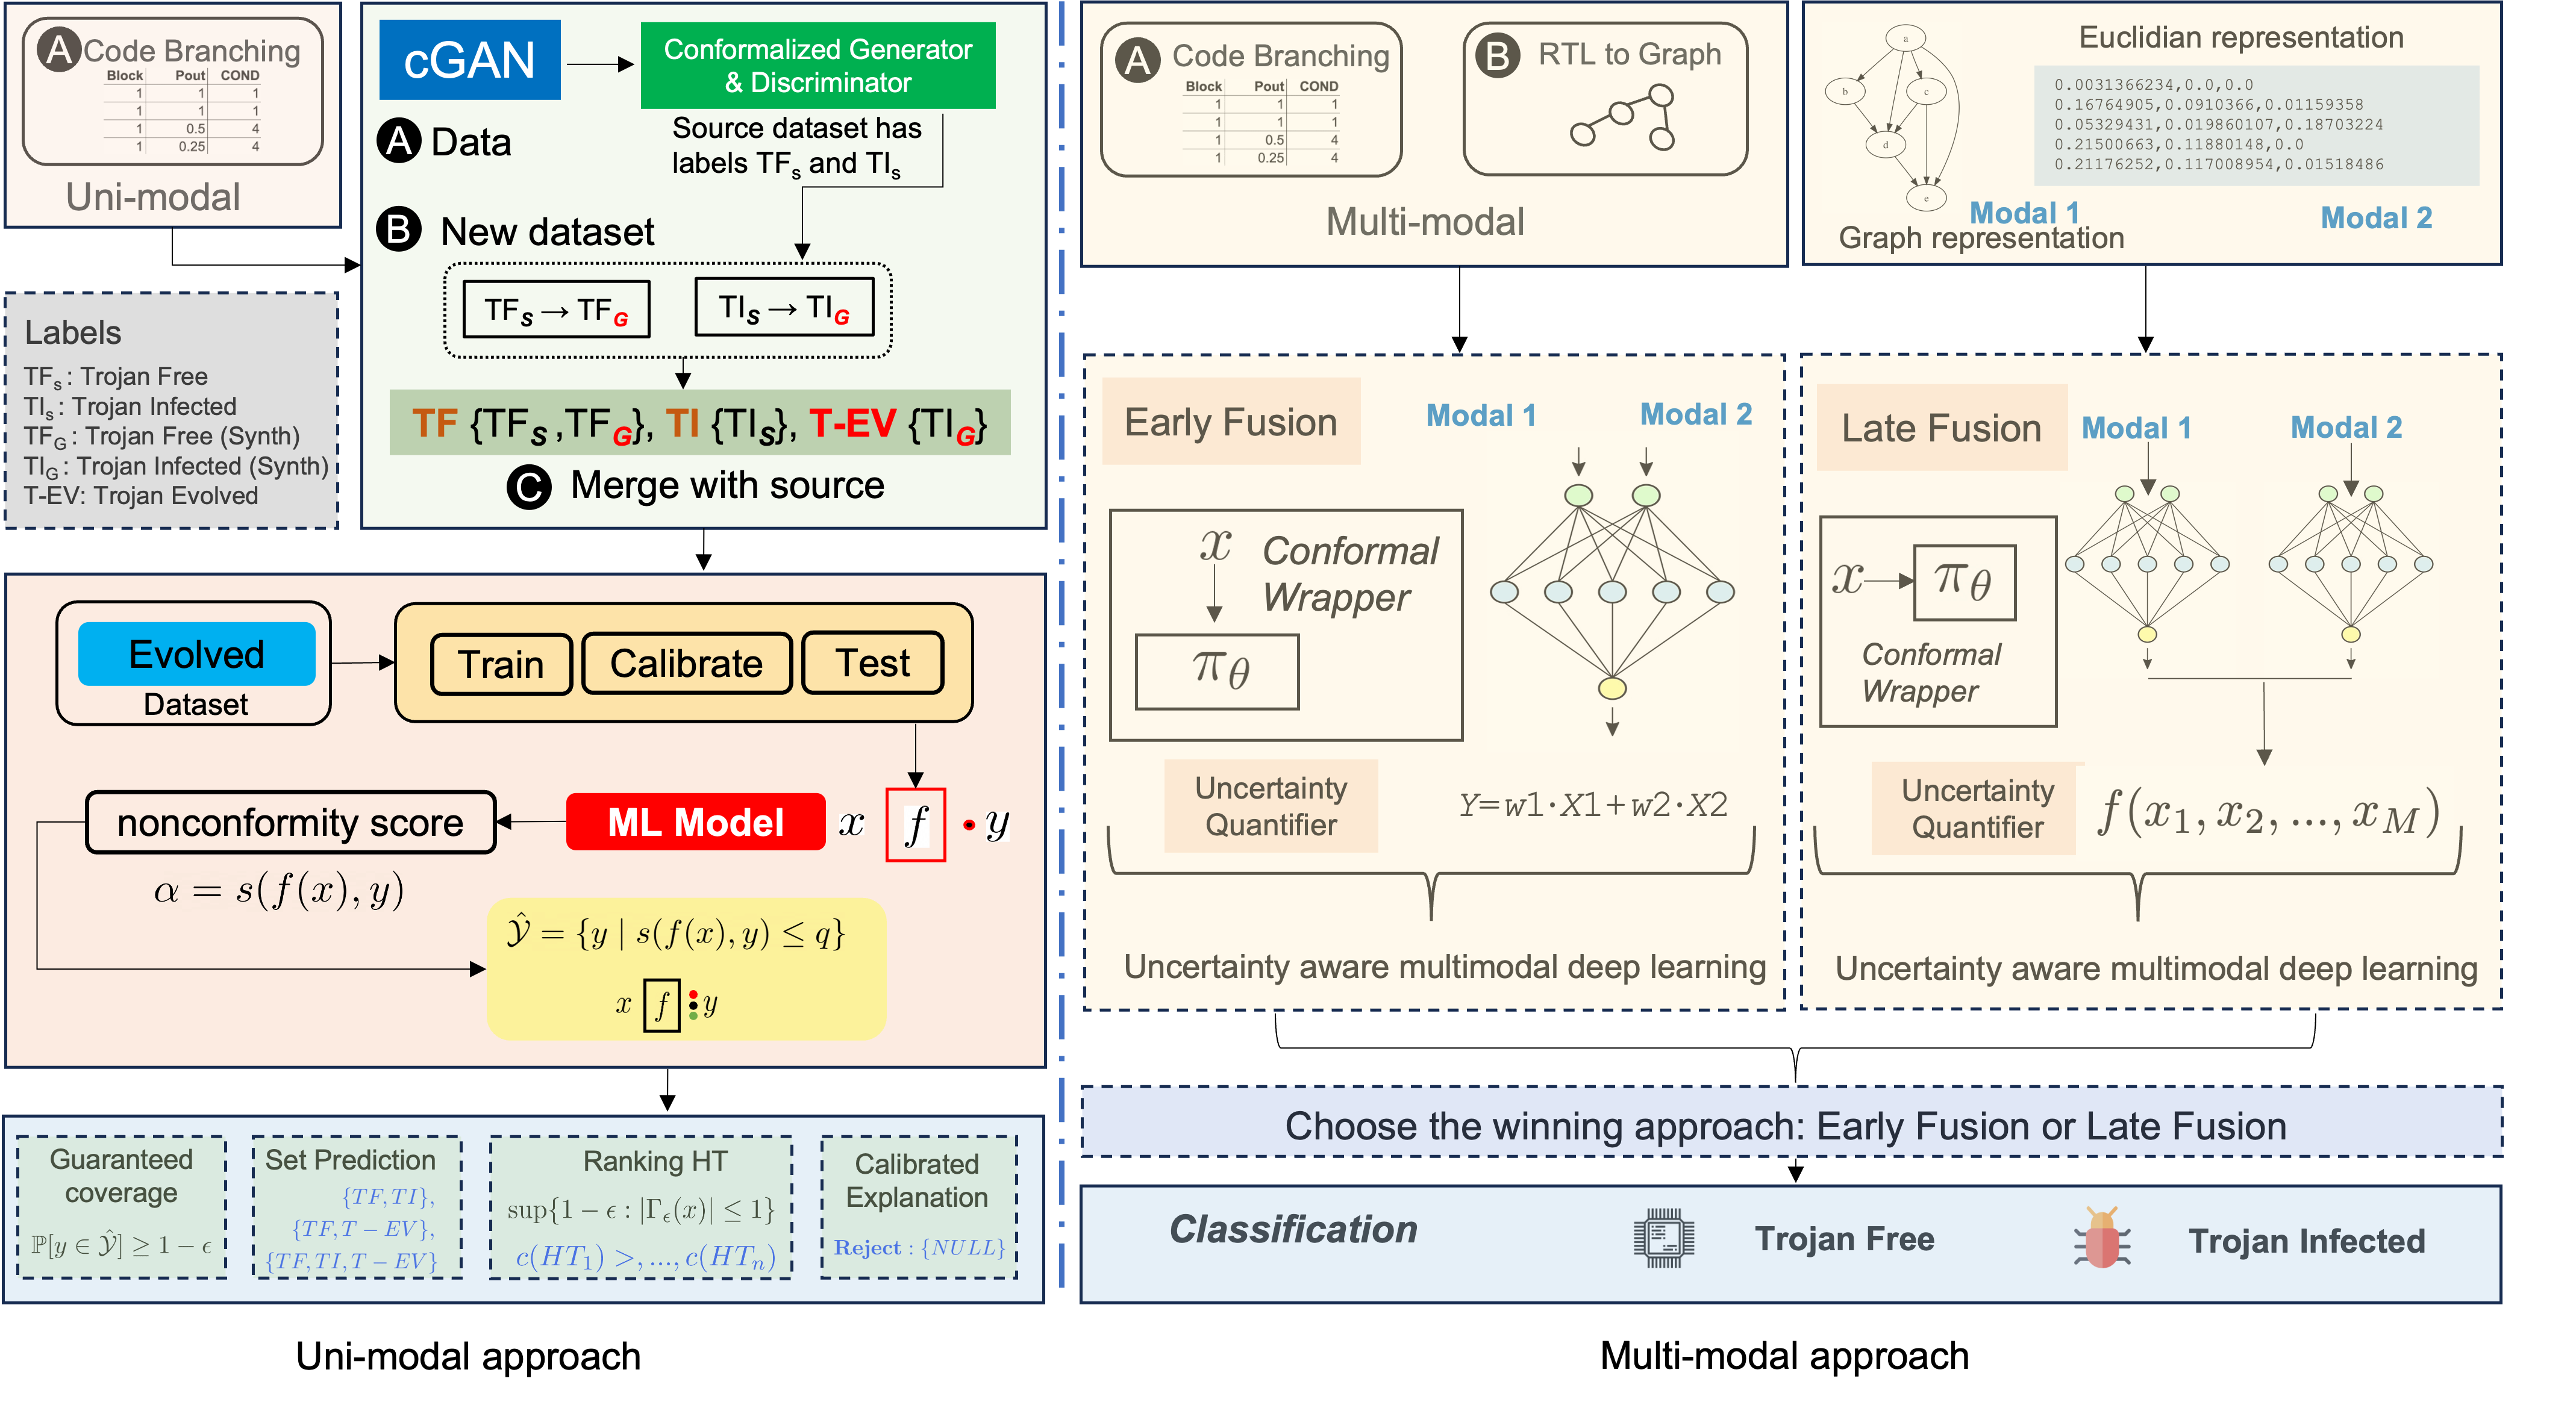
\includegraphics[width=1\linewidth]{figs/solution_thesis.png}
   \caption{The input feature is passed to a conventional machine learning hardware Trojan detector. This detector produces a result and is compared to conformal inference, which provides an uncertainty measure and a confidence set for each detected evolved hardware Trojan.}
  \label{fig:introduction}
\end{figure}


\section*{Contributions}
\label{Contribution}
In this thesis, our primary focus revolves around multimodal deep learning for the identification of hardware trojans, and addressing the inherent challenges associated with this problem, for example, missing modalities and imbalanced dataset. The first challenge pertains to effectively handling missing modalities and implementing uncertainty-aware multimodal fusion approaches. To address this, we utilize graphical representations of circuits \cite{yu2021hw2vec} and Euclidean data derived from processing the Abstract Syntax Tree (AST) of RTL files (Verilog) \cite{px6s-sm21-22}. While multimodal approaches have been employed to enhance model accuracy in various domains, their application in Trojan identification has been notably absent. For uncertainty-aware multimodal learning, we advocate for implementing logic at the information fusion level of modalities, leveraging $p$-values aggregation with conformal prediction.

The second challenge we tackle is the quantification of uncertainty associated with hardware trojan prediction outcomes and ensuring the validity of predicted labels, especially when dealing with a limited number of highly imbalanced data points. Specifically, our interest lies in the ability of a machine learning classifier to predict the true label of a new data point with a 95\% provable guaranteed coverage, a crucial requirement in risk-sensitive domains. Designing such a system holds potential benefits for decision-makers investigating detected labels as "Trojan-Infected." Additionally, we explore the possibility of ranking detected "Trojan-Infected" circuits to enable more informed treatment decisions.

Our primary contributions are summarized as follows:

\begin{itemize}
\item Proposing a multimodal learning approach using graph and Euclidean data of the hardware circuits. This study is the first to investigate and implement a multimodal approach for HT detection, emphasizing uncertainty-awareness.
\item Suggesting a model fusion approach that leverages $p$-values as statistical measures, systematically assessing each modality's contribution to the overall prediction. This enhances interpretability and facilitates more robust decision-making.
\item Addressing the challenges of missing modalities and solving the issue of handling an imbalanced and small dataset by leveraging generative adversarial networks.
Introducing the notion of HT evolution and providing an innovative method of creating evolving HTs with high precision using a conformalized generative adversarial network.
\item Novel concept of guaranteed coverage of the prediction set, proposing a tunable significance level through conformal prediction for HT detection. Additionally, defining an algorithm-agnostic and explainability-aware reject prediction made by the ML model. When the model is uncertain about identifying the evolving Trojan, it rejects the prediction, passing it to a human for manual investigation.
\item Proposing a ranking mechanism for the evolved Trojans by assigning a confidence score from the prediction. This contribution is validated on synthetic and real chip-level HT-induced benchmarks.
\end{itemize}


\endgroup